\documentclass[../ASSD_TP2.tex]{subfiles}
\begin{document}
\section*{Síntesis basada en muestras}
\subsection*{Introducción}
El objetivo de la síntesis basada en muestras es poder conseguir distintas notas y duración de un instrumento, a partir de una muestra. Para lograrlo basta con resolver uno de dos problemas:
\begin{itemize}
\item Alterar la frecuencia fundamental si modificar la duración
\item Modificar la duración sin alterar la frecuencia fundamental
\end{itemize}

Solucionado uno de los previamente mencionado vasta resamplear la se\~nal con una frecuencia distintas. Por ejemplo si se resamplea a una frecuencia de sampleo del doble, se alteraría la frecuencia fundamental pero también la duración, por ende bastaría con alargarlo en el tiempo sin alterar la frecuencia.
\subsection*{TME(Time Scale Modification)}
Tal como su nombre lo indica, refiere  algoritmos con la capacidad de alterar la longitud temporal de una muestra. El algoritmo mas sencillo capaz de lograrlo es el resampling:

\begin{lstlisting}
def resampling(x,Fs,scale):
	y=interpolate(x)
	y=sample(y,scale*Fs)
	return y
\end{lstlisting}
A pesar de su sencillez el problema fundamental de este algoritmos es que altera las frecuencias de las muestras. Por ende para evitar este problema se requieren algoritmos mas complejos.
\subsubsection*{OLA(Overlap and add)}
El principio de funcionamiento del algoritmo, es tomar segmentos del fragmento original y superponerlos hasta obtener la longitud deseada.

\begin{figure}[H]
  \centering
   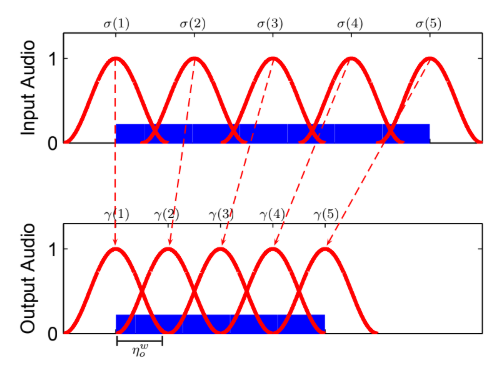
\includegraphics[width=0.5\textwidth]{figures/ola.png}
  \caption{Ejemplo del funcionamiento del algoritmo, imagen obtenida de Driedger Jonathan TSM Master Thesis}
\end{figure}
El primer paso del algoritmo es fraccionar el segmento original, a cada fragmento se le aplica una ventana de tipo Hann. Posteriormente se los superponen el el nuevo fragmento. El estiramiento lo produce una función que convierte las posiciones de un segmento al otro.
\par Matemáticamente el algoritmo se puede describir de la siguiente manera:
\begin{equation}
y(n)=\frac{\sum_{k=1}^{len(\sigma)} \omega(n - \gamma (k)) x(n-\gamma (k) + \sigma (k))}{\sum_{k=1}^{len(\sigma)}\omega(n - \gamma (k))}
\end{equation}
Donde $\sigma$ es un vector de indices correspondiente a la entrada, $\gamma$ es un vector de indices correspondiente a la salida. La función que los vincula es $\tau$, dicha función convierte los indices en el intervalo de entrada al intervalo de salida.
$\omega$ es el vector que contiene los valores de la ventana en cada punto, el ancho de la ventana $\omega l$ tiene que ser mas grande que el periodo de la se\~nal de menor frecuencia.

\par El algoritmo funciona correctamente para se\~nales cuya naturaleza sea no armónica, por ejemplo el habla. Sin embargo para se\~nales armónicas introduce modulación, y saltos de fase, a los desfajases producidos en el overlapping de las muestras.  

\begin{figure}[H]
 \centering
  \subfloat[Tiempo]{
   %\label{f:ejaesc}
    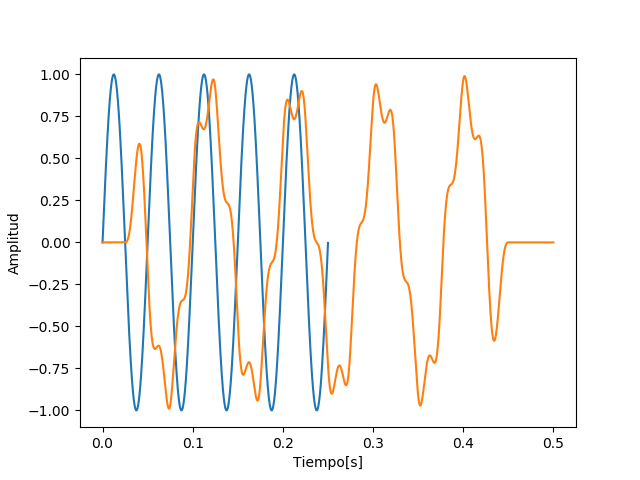
\includegraphics[width=0.48\textwidth]{figures/x2.png}}
  \subfloat[Espectro]{
   %\label{f:ejaimp}
    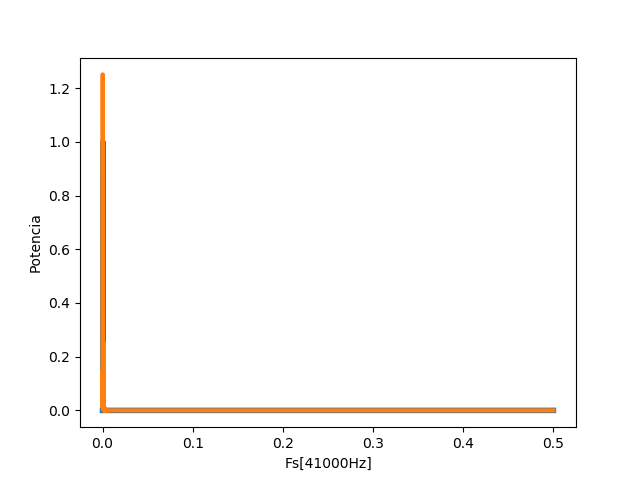
\includegraphics[width=0.48\textwidth]{figures/fftx2.png}}

 \caption{Resultados del algoritmo, factor de escalamiento 2, se\~nal senoidal de 20 Hz. La se\~nal naranja corresponde a la salida y la azul a la entrada}
 %\label{f:eja}
\end{figure}

\begin{figure}[H]
 \centering
  \subfloat[Tiempo]{
   %\label{f:ejaesc}
    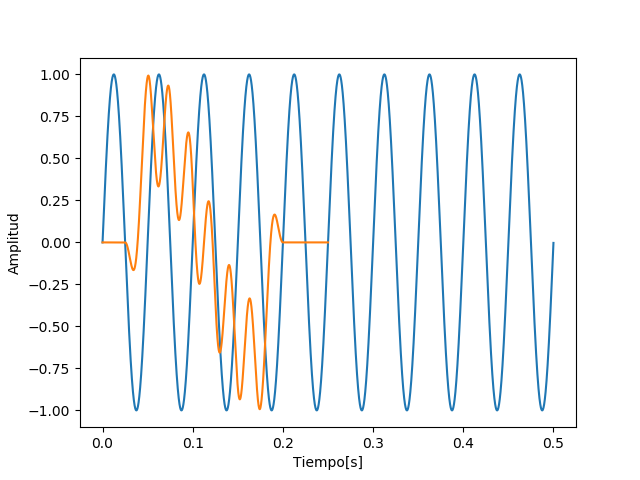
\includegraphics[width=0.48\textwidth]{figures/xmit.png}}
  \subfloat[Espectro]{
   %\label{f:ejaimp}
    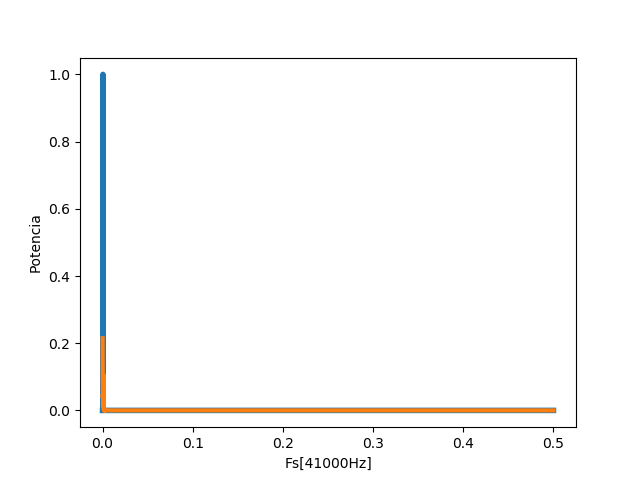
\includegraphics[width=0.48\textwidth]{figures/fftxmit.png}}

 \caption{Resultados del algoritmo, factor de escalamiento $\frac{1}{2}$, se\~nal senoidal de 20 Hz. La se\~nal naranja corresponde a la salida y la azul a la entrada}
 %\label{f:eja}
\end{figure}

Tal como era des esperarse el algoritmo introduce modulación a se\~nales armónicas, este fenómeno se ve realizando un acercamiento a la FFT

\begin{figure}[H]
  \centering
   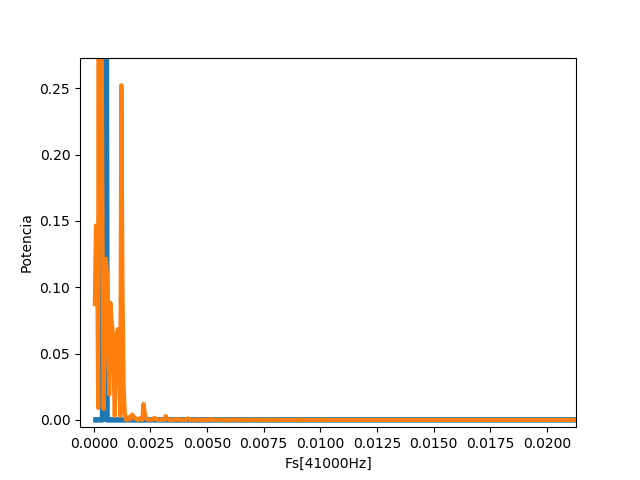
\includegraphics[width=0.5\textwidth]{figures/zoom.png}
  \caption{Acercamiento de la FFT, factor de escalamiento 2}
\end{figure}

\subsubsection*{WSOLA(Wave Similarity Overlap and Add)}
El funcionamiento del algoritmo es similar al OLA, intenta solucionar el problema de las se\~nales armónicas. El problema de OLA, radica en que realiza siempre la misma acción independientemente de la se\~al de entrada.
\par Para solucionar el problema WSOLA, varia el la posición que toma del fragmento original un $\Delta K$.

\begin{figure}[H]
  \centering
   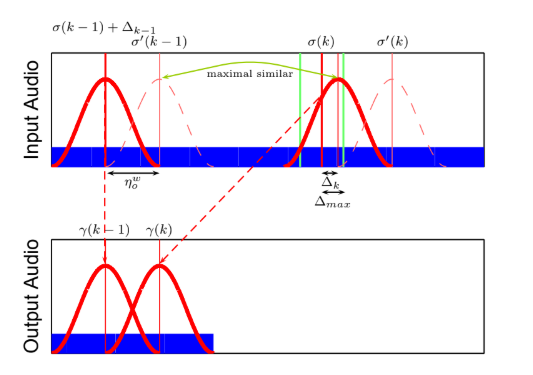
\includegraphics[width=0.7\textwidth]{figures/wsola.png}
  \caption{Ejemplo del funcionamiento del algoritmo, imagen obtenida de Driedger Jonathan TSM Master Thesis}
\end{figure}

Matemáticamente se describe similar al OLA salvo por offset.
\begin{equation}
y(n)=\frac{\sum_{k=1}^{len(\sigma)} \omega(n - \gamma (k)) x(n-\gamma (k) + \sigma (k) + \Delta K)}{\sum_{k=1}^{len(\sigma)}\omega(n - \gamma (k))}
\end{equation}

El $\Delta K$ se obtiene haciendo la correlación cruzada(busca similitud, para evitar saltos de fase) entre dos fragmentos contiguos en la entrada.

\subsection*{PSOLA(Pitch Synchronous Overlap and Add)}





\end{document}
